% !TEX TS-program = pdflatex
% !TEX encoding = UTF-8 Unicode

% This is a simple template for a LaTeX document using the "article" class.
% See "book", "report", "letter" for other types of document.

\documentclass[14pt]{article} % use larger type; default would be 10pt

\usepackage[utf8]{inputenc} % set input encoding (not needed with XeLaTeX)

%%% Examples of Article customizations
% These packages are optional, depending whether you want the features they provide.
% See the LaTeX Companion or other references for full information.

%%% PAGE DIMENSIONS
\usepackage{geometry} % to change the page dimensions
\geometry{a4paper} % or letterpaper (US) or a5paper or....
% \geometry{margin=2in} % for example, change the margins to 2 inches all round
% \geometry{landscape} % set up the page for landscape
%   read geometry.pdf for detailed page layout information

\usepackage{graphicx} % support the \includegraphics command and options

% \usepackage[parfill]{parskip} % Activate to begin paragraphs with an empty line rather than an indent
\usepackage{float}
\usepackage{titling}
%%% PACKAGES
\usepackage{booktabs} % for much better looking tables
\usepackage{array} % for better arrays (eg matrices) in maths
\usepackage{paralist} % very flexible & customisable lists (eg. enumerate/itemize, etc.)
\usepackage{verbatim} % adds environment for commenting out blocks of text & for better verbatim
\usepackage{subfig} % make it possible to include more than one captioned figure/table in a single float
% These packages are all incorporated in the memoir class to one degree or another...

%%% HEADERS & FOOTERS
\usepackage{fancyhdr} % This should be set AFTER setting up the page geometry
\pagestyle{fancy} % options: empty , plain , fancy
\renewcommand{\headrulewidth}{0pt} % customise the layout...
\lhead{}\chead{}\rhead{}
\lfoot{}\cfoot{\thepage}\rfoot{}

%%% SECTION TITLE APPEARANCE
\usepackage{sectsty}
\allsectionsfont{\sffamily\mdseries\upshape} % (See the fntguide.pdf for font help)
% (This matches ConTeXt defaults)

%%% ToC(table of contents) APPEARANCE
\usepackage[nottoc,notlof,notlot]{tocbibind} % Put the bibliography in the ToC
\usepackage[titles,subfigure]{tocloft} % Alter the style of the Table of Contents
\renewcommand{\cftsecfont}{\rmfamily\mdseries\upshape}
\renewcommand{\cftsecpagefont}{\rmfamily\mdseries\upshape} % No bold!
\geometry{margin=1.5in}
%%% END Article customizations

%%% The "real" document content comes below...



%\date{} % Activate to display a given date or no date (if empty),
         % otherwise the current date is printed 

\begin{document}
\tableofcontents

\pagebreak
\title{CHAPTER 1}
\maketitle
\section{INTRODUCTION}

\subsection{INTRODUCTION}
         Radar systems are generally used in determining properties, most commonly distance from a reference point, of solid objects using single antennas or large antenna arrays. These antennas transmit and receive electromagnetic signals, which can be processed to obtain various relevant data. By using only one antenna and moving it along a linear axis to record an area of static objects, one can mimic a larger array of antennas to collect high-resolution data: this setup is known as a synthetic aperture radar system. The data collected from this type of radar configuration, after processing, is well-known for its detail and map-like quality, and can be used to render a two-dimensional and three-dimensional representation of scanned area.

\subsection{PROBLEM STATEMENT}
           Radars produce large amounts of data and this has important implications for the archiving and analysis of data. The need for methods to deal with radar data sets will only increase as DRDO is developing multiple sided radar under their project QRSAM. Till now Radar data has been processed in a very traditional manner by going through each bit of big binary files. So, each time whenever an information about particular dwells were needed, it involved a long task of searching each binary files and getting the information. Also the raw radar data contain lot of garbage data which makes it difficult and tedious task to test radar during its development phase. The brute force approach of reading data every time when needed from raw files, uncompressing the data, analysing, loading another chunk, and so on, is impractical. For one, it limits access to the data and prevents parallel research activities.

\subsection{OBJECTIVE}
 To develop a software capable of handling large raw binary radar data and reading each dwells and saving information in a database. Also the software should be capable of reading multiple data without any loss in dwells information and can exclude garbage data. The software should be able to extract clean required radar data and merge it to files. The final objective of this project includes its analysis and the algorithm devised should be fast enough to process large data at real time. 
 
 \pagebreak
 \subsection{STEPS INVOLVED}
 \begin{figure}[H]
  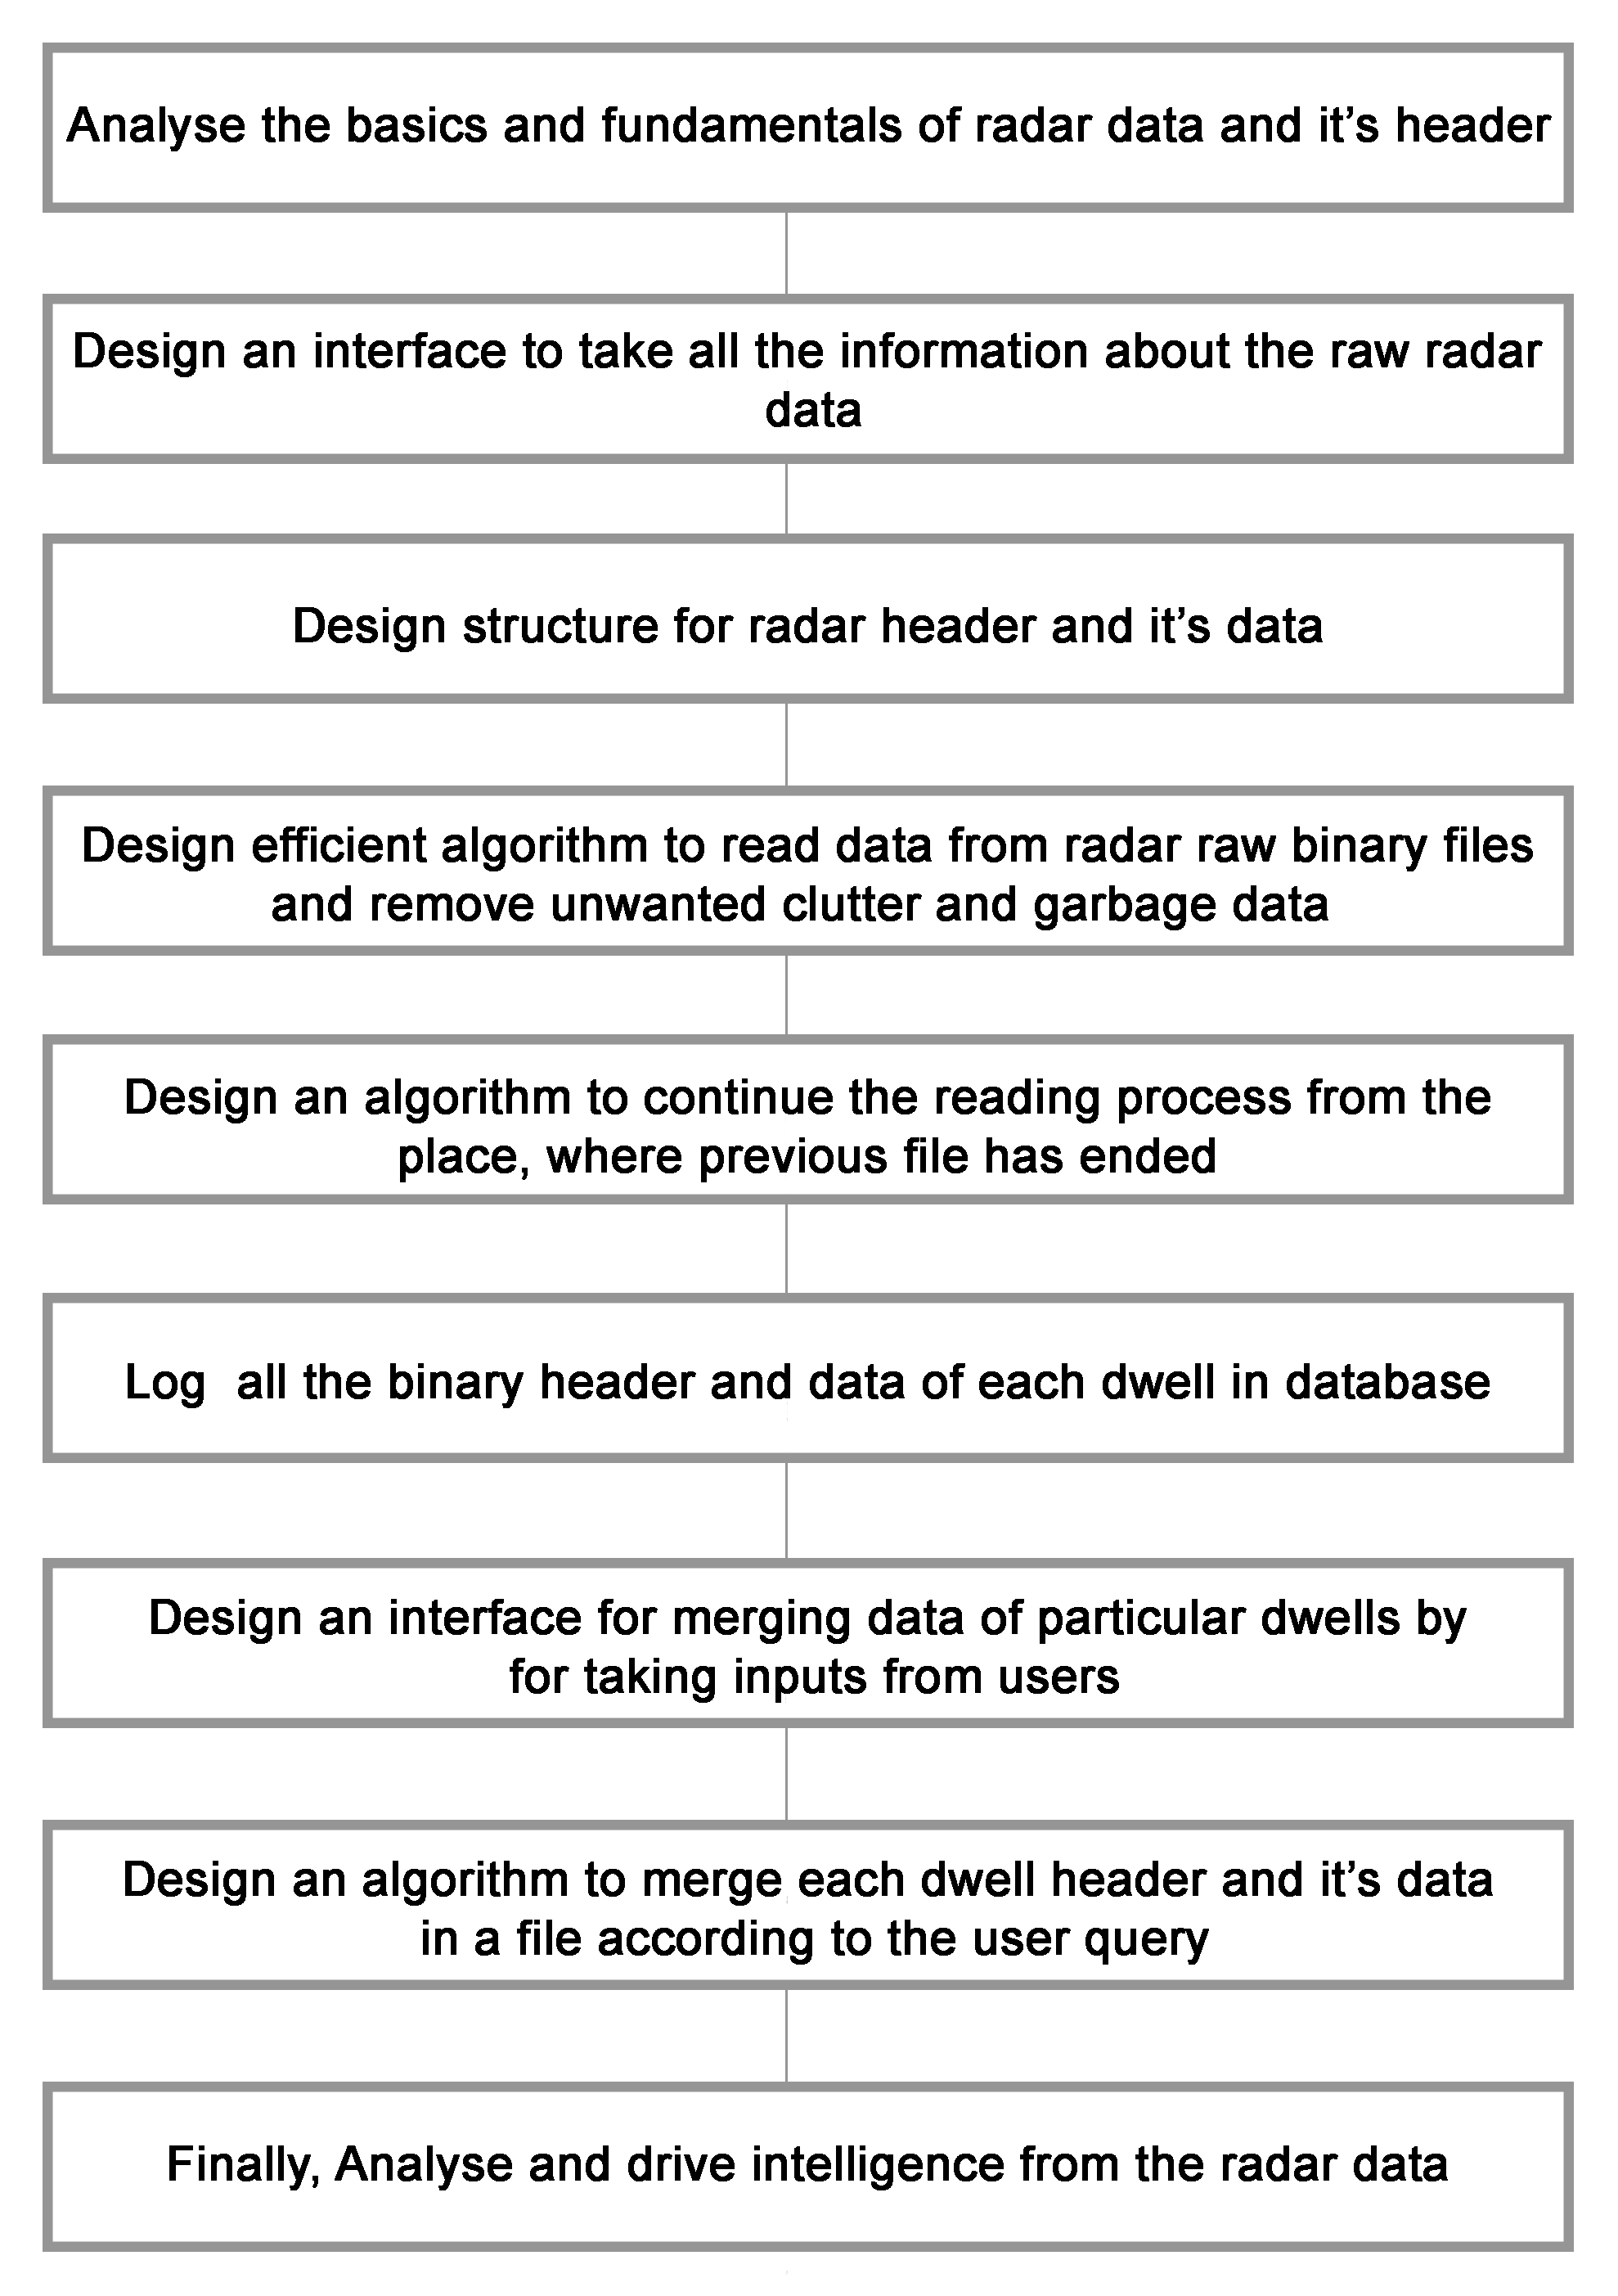
\includegraphics[width=\linewidth]{steps.png}
  \caption{Steps involved.}
  \label{fig:figure 1}
\end{figure}

\subsection{CONSTRAINTS}
Data collected from radars are voluminous. For example, a single volume of radar reflectivity data from the QRSAM, BSR radar requires about   1 GB of disk space. With a volume collected approximately every 30 minutes, this corresponds to 48 GB per day if operated for one day. Archiving and processing such large data sets every time are formidable tasks. The brute force approach of reading data every time when needed from raw files, uncompressing the data, analysing, loading another chunk, and so on, is impractical. For one, it limits access to the data and prevents parallel research activities.

\pagebreak

\title{CHAPTER 2}
\maketitle
\section{ABOUT LRDE, DRDO}

\subsection{ABOUT ORGANISATION}
\textbf{ELECTRONICS AND RADAR DEVELOPMENT ESTABLISHMENT (LRDE)} is one among the labs under \textbf{ Defence Research and Development Organization (DRDO)}. Defence Research \& Development Organisation (DRDO) works under Department of Defence Research and Development of Ministry of Defence. LRDE has its genesis in the Inspectorate of Scientific Stores created in 1939 at  Rawalpindi which was re-designated as Technical Development Establishment (Instruments and Electronics) in 1946 and located at Dehradun. In the year 1958 the Electronics Research and Development Establishment was formed at Bangalore with men and material inherited from TDE (I\&E).. 

\subsection{CORE COMPETENCIES}
\begin{itemize}
 \item	Design and Development of major sub-systems - Mechanical and Electronic Scanning Antennas, High Performance Transmitters, Exciters, Receivers, T/R Modules, Digital Signal \& Data Processors, Mechanical Engineering.
\item	Radar System Engineering for Ground based, Ship borne and Air borne systems.
\item	Environmental engineering including EMI/EMC.
\item	Radar System Integration and Evaluation
\end{itemize}
\subsection{ACTIVITIES}
Design and Development of Radar Systems are
\begin{enumerate}
\item 
\textbf{Army}
\begin{itemize}
\item	Multifunction Phased Array Radar and 3D Surveillance Radar for Akash Missile Weapon System.
\item	 Low Level 2D Radar for Fire Control and Air Defence.
\item	 Short Range Battle Field Surveillance Radar.
\item	 Weapon Locating Radar.
\item	 3D Tactical Control Radar.
	 \end{itemize}
\item
\textbf{Navy}
\begin{itemize}
\item	Maritime Patrol Radar for fixed and Rotary Wing Aircraft.
\item	Maritime Patrol Radar with SAR \& ISAR.
\item	 3D Medium Range Surveillance Radar for ASW Corvettes
\end{itemize}
\item
\textbf{Airforce}
\begin{itemize}
\item	Multifunction Phased Array Radar and 3D Surveillance Radar for Akash Missile Weapon System.
\item	Active Phased Array Radar for AEW\&C.
\item	Low level 2D radar and 3D Short \& Medium Range Surveillance Radar for Air Defence.
\item	Medium Power Radar (MPR).
\item	 Low Level Transportable Radar (LLTR).
\item	Active Electronically Scanned Array Radar (AESA).
\end{itemize}

\end{enumerate}

\pagebreak

\title{CHAPTER 3}
\maketitle
\section{ABOUT RADAR}
\subsection{RADAR FUNDAMENTALS}
Radar is acronym for Radio Detection and Ranging. Radar is an electromagnetic system for detection and location for reflecting objects. Radar can also be used to detect stationary objects buried underground. In some cases, Radar can identify as well .For example, it can identify the type of the aircrafts it has detected. It operates by radiating energy into space and detecting the eco signal reflected from an object or target. The reflected energy that is returned to the radar not only indicates the presence of a target, but by comparing received echo signal with the signal that was transmitted, its location can be determined along with other target related information. Radar can perform its functions at long or short distance and  under conditions improvises to optical and infrared sensors. Its ability to measure distance with high accuracy and weather is one of its most important attributes. The radar makes use of radio waves that are electromagnetic in nature which gets reflected when they encounter some object in their path. 
The time taken by the radio waves to go from the transmitter to the objects and in coming back to the receiver is recorded by Radar, which is used to determine the distance of objects from the Radar by the simple equation given by
 \begin{center}                                             
    R=CT/2
 \end{center}
Where R is range of the target from the Radar.
 C is speed of the electromagnetic wave which is equal to the velocity.
 T is time taken by the pulse to travel from transmitter to target and back from target to receiver.
\subsection{RADAR BLOCK DIAGRAM}
 The block diagram given below Figure 2 shows the main components of the basic radar system and their operations are:
\begin{itemize}

\item \textbf {\underline{Transmitter}:}
\\* The radar transmitter produces the short duration high-power rf pulses of energy that are into space by the antenna.
\item \textbf {\underline{Duplexer}:}
 \\*     The duplexer alternately switches the antenna between the transmitter and receiver so that only one antenna need be used. This switching is necessary because the high-power pulses of the transmitter would destroy the receiver if energy were allowed to enter the receiver.
      
\begin{figure}[H]
  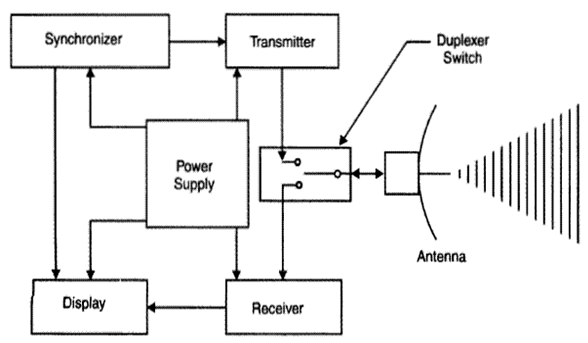
\includegraphics[width=\linewidth]{RadarBlockDiagram.png}
  \caption{Block diagram of radar.}
  \label{fig:figure 2}
\end{figure}


\item \textbf {\underline{Receive}:}
 \\*     The receivers amplify and demodulate the received RF-signals. The receiver provides video signals on the output.
\item \textbf {\underline{Radar-Antenna}:}
 \\*     The Antenna transfers the transmitter energy to signals in space with the required distribution and efficiency. This process is applied in an identical way on reception.
\item \textbf {\underline{Indicator}:}
\\* The indicator should present to the observer a continuous, easily understandable, graphic picture of the relative position of radar targets. The radar screen (in this case a PPI-scope) displays the produced from the echo signals bright blips. The longer the pulses were delayed by the runtime, the further away from the canter of this radar scope they are displayed. The direction of the deflection on this screen is that in which the antenna is currently pointing.
\end{itemize}
\subsection{RADAR FREQUENCY BANDS}
The following Table 1 shows radar frequency bands:

 

High Frequency (HF) radars utilize the electromagnetic waves’ reflection off the ionosphere to detect targets beyond the horizon. Some examples include the United States over the Horizon Backscatter (U.S. OTH/B) radar which operates in the frequency range of, the U.S. Navy Reloadable Over The Horizon Radar (ROTHR), see Fig. 2.3-2, and the Russian Woodpecker radar. Very High Frequency (VHF) and Ultra High Frequency (UHF) bands are used for very long range Early Warning Radars (EWR). Some examples include the Ballistic Missile Early Warning System (BMEWS) search and track mono-pulse radar which operates at (Fig. 2.3-3), the Perimeter and Acquisition Radar (PAR) which is a very long range multifunction phased
array radar, and the early warning PAVE PAWS multifunction UHF phased array radar. Because of the very large wavelength and the sensitivity requirements for very long range measurements, large apertures are needed in such radar systems.


 \begin{figure}[H]
  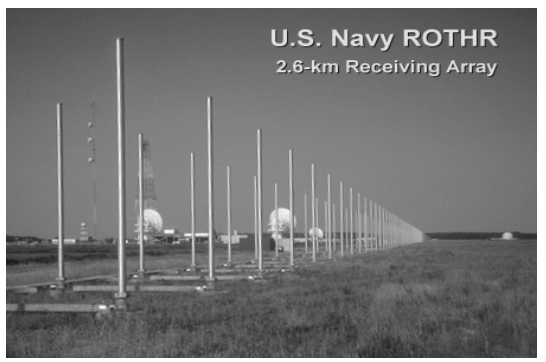
\includegraphics[width=\linewidth]{Horizonradar.png}
  \caption{U. S. Navy Over The Horizon Radar}
  \label{fig:figure 4}
\end{figure}
Radars in the L-band are primarily ground based and ship based systems that are used in long range military and air traffic control search operations. Most ground and ship based medium range radars operate in the S-band. For example, the Airport Surveillance Radar (ASR) used for air traffic control, and the ship based U.S. Navy AEGIS (Fig. 2.6-4) multifunction phased array are S-band radars. The Airborne Warning And Control System (AWACS) shown in Fig. 2.6-5 and the National Weather Service Next Generation Doppler Weather Radar (NEXRAD) are also S-band radars. However, most weather detection radar systems are C-band radars. Medium range search and fire control military radars and metric instrumentation radars are also C-band.


 \begin{figure}[H]
  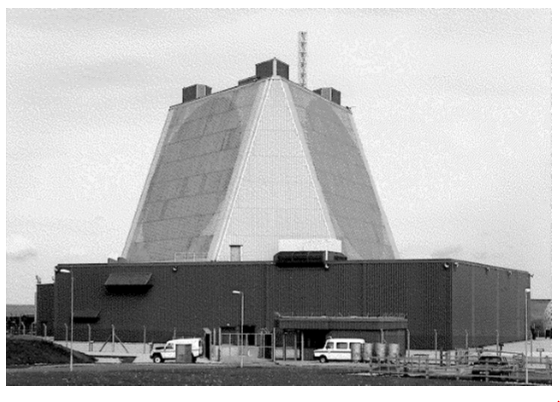
\includegraphics[width=\linewidth]{fylingdales.png}
  \caption{Fylingdales BMEWS - United Kingdom}
  \label{fig:figure 5}
\end{figure}


\begin{figure}[H]
  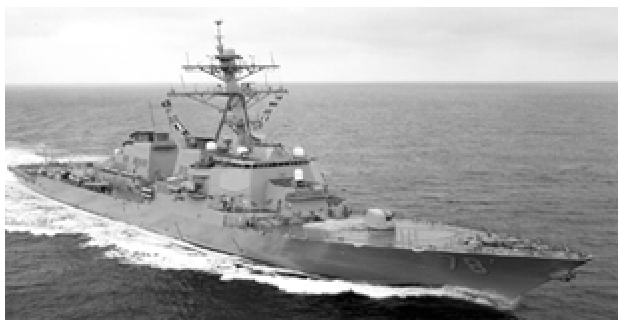
\includegraphics[width=\linewidth]{Navy.png}
  \caption{U. S. Navy AEGIS}
  \label{fig:figure 6}
\end{figure}
\end{document}
